%!TEX root = ../Theory.tex

\section{Snoek's limit} % (fold)
\label{sec:snoek_s_limit}

\begin{align*}
	\pqty{\mu_0^\prime - 1} f_0 = \frac{2}{3}\gamma 4\pi M_s
\end{align*} where $4\pi M_s$ is the saturation magnetization and $\gamma \approx \SI{3}{MHz/Oe}$.

% section snoek_s_limit (end)

\section{Reflectometry} % (fold)
\label{sec:reflectometry}

\subsection{This} % (fold)
\label{sub:this}

\begin{align*}
	R\pqty{q_z} = R_F\abs{\frac{1}{\rho_S}\int \eval{\dv{\rho}{z}}_z e^{-iq_z z}\dd{z}}^2
\end{align*}

% subsection this (end)

\subsection{That} % (fold)
\label{sub:that}

% subsection that (end)

The propagation of light as a magneto-electric wave of wave vector $\vb{k}$ is given by,
\begin{align*}
	\vb{E}\pqty{\vb{r},t} &= \vb{E}_{0}e^{i\pqty{\vb{k}\cdot\vb{r} - \omega t}} & \vb{B}\pqty{\vb{r},t} &= \frac{\vu{k}\times\vb{E}\pqty{\vb{r},t}}{v}
\end{align*}

\begin{align*}
	\vb{E}\pqty{\vb{r},t} &= \vb{E}_{0}e^{i\pqty{\vb{k}\cdot\vb{r} - \omega t}} & \omega \vb{B}\pqty{\vb{r},t} &= \vb{k}\times\vb{E}\pqty{\vb{r},t}
\end{align*}

In each layer $j$, there is a wave incident \text{(I)} and a reflected \text{(R)} wave,
% \begin{align*}
% 	\vb{E}_j\pqty{\vb{r},t} &= 
% 		\vb{E}_{0j}^{\text{(I)}}e^{i\pqty{\vb{k}_j^{\text{(I)}}\cdot\vb{r} - \omega t}} + 
% 		\vb{E}_{0j}^{\text{(R)}}e^{i\pqty{\vb{k}_j^{\text{(R)}}\cdot\vb{r} - \omega t}} \\
% 	\omega\vb{B}_j\pqty{\vb{r},t} &= 
% 		\vb{k}_j^{\text{(I)}}\times\vb{E}_{0j}^{\text{(I)}}e^{i\pqty{\vb{k}_j^{\text{(I)}}\cdot\vb{r} - \omega t}} + 
% 		\vb{k}_j^{\text{(R)}}\times\vb{E}_{0j}^{\text{(R)}}e^{i\pqty{\vb{k}_j^{\text{(R)}}\cdot\vb{r} - \omega t}}
% \end{align*}
\begin{align*}
	\vb{E}_j\pqty{\vb{r},t} &= 
		\bqty{
			\vb{E}_{0j}^{(\text{I})}\exp\pqty{i\vb{k}_j^{(\text{I})}\cdot\vb{r}} + 
			\vb{E}_{0j}^{(\text{R})}\exp\pqty{i\vb{k}_j^{(\text{R})}\cdot\vb{r}}
		} e^{-i \omega t}\\
	\omega\vb{B}_j\pqty{\vb{r},t} &= 
		\bqty{
			\vb{k}_j^{(\text{I})}\times\vb{E}_{0j}^{(\text{I})}\exp\pqty{i\vb{k}_j^{(\text{I})}\cdot\vb{r}} + 
			\vb{k}_j^{(\text{R})}\times\vb{E}_{0j}^{(\text{R})}\exp\pqty{i\vb{k}_j^{(\text{R})}\cdot\vb{r}}
		} e^{-i \omega t}
\end{align*}

Wave vector and group speed are related,
\begin{align*}
	k_j^{\text{(I,R)}}v_j &= \omega & k_j^{\text{(I,R)}} = \abs*{\vb{k}_j^{\text{(I,R)}}}
\end{align*}

\begin{align*}
	n_j v_j &= c & \frac{n_j}{k_j^{\text{(I,R)}}} &= \frac{c}{\omega} = \frac{\lambda}{2\pi}
\end{align*}

% \begin{align*}
% 	\vb{E}_{j-1}\pqty{\vb{r}_j,t} &= \vb{E}_{j}\pqty{\vb{r}_j,t} \\
% 	\vb{B}_{j-1}\pqty{\vb{r}_j,t} &= \vb{B}_{j}\pqty{\vb{r}_j,t}
% \end{align*}

\begin{figure}
\begin{center}
    {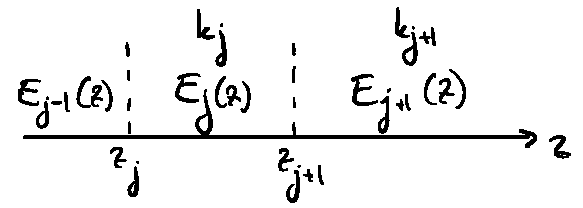
\includegraphics{Figures/SpaceDiscretion.pdf}
    }
\caption{
Caption
}
\label{fig:1}
\end{center}
\end{figure}

The interface between layer $j-1$ and $j$ is define as $\boldsymbol{\mathsf{r}}_j$. 
\begin{align*}
	\boldsymbol{\mathsf{r}}_j = x\vu{x} + y\vu{y} + z_j\vu{z}
\end{align*}
The electric field component at the interface need to respect the following equation
\begin{align*}
	\pqty{\vb{E}_{j-1}\pqty{\boldsymbol{\mathsf{r}}_j,t}}_{x,y} &= \pqty{\vb{E}_{j}\pqty{\boldsymbol{\mathsf{r}}_j,t}}_{x,y} \\
	\epsilon_{j-1}\pqty{\vb{E}_{j-1}\pqty{\boldsymbol{\mathsf{r}}_j,t}}_z &= \epsilon_{j}\pqty{\vb{E}_{j}\pqty{\boldsymbol{\mathsf{r}}_j,t}}_z
\end{align*} while the magnetic field components,
\begin{align*}
	\frac{1}{\mu_{j-1}}\pqty{\vb{B}_{j-1}\pqty{\boldsymbol{\mathsf{r}}_j,t}}_{x,y} &= \frac{1}{\mu_j}\pqty{\vb{B}_{j}\pqty{\boldsymbol{\mathsf{r}}_j,t}}_{x,y} \\
	\pqty{\vb{B}_{j-1}\pqty{\boldsymbol{\mathsf{r}}_j,t}}_z &= \pqty{\vb{B}_{j}\pqty{\boldsymbol{\mathsf{r}}_j,t}}_z 
\end{align*}

Note that, at the frequency of X rays, the relative magnetic permeabilty of matter is unity up to many orders of magnitude, (Snoek's limit)
\begin{align*}
	\mu_j \sim \mu_0 && \frac{\Delta \mu}{\mu_0} \ll \frac{\Delta \epsilon}{\epsilon_0}
\end{align*} 

As an example, the continuity of the $x$ component of the electric field gives the following equation,
\begin{align*}
		E_{0z,{j-1}}^{(\text{I})}\exp\pqty{i\vb{k}_{j-1}^{(\text{I})}\cdot\vb{r}} + 
		E_{0z,{j-1}}^{(\text{R})}\exp\pqty{i\vb{k}_{j-1}^{(\text{R})}\cdot\vb{r}}
	&= 
		E_{0z,j}^{(\text{I})}\exp\pqty{i\vb{k}_j^{(\text{I})}\cdot\vb{r}} + 
		E_{0z,j}^{(\text{R})}\exp\pqty{i\vb{k}_j^{(\text{R})}\cdot\vb{r}}
\end{align*}

% All these equation will have phase factors that must connect at the interface. 
% \begin{align*}
% 	\exp i\pqty{k^{\text{\text{(I)}}}_{x,j}x + k^{\text{\text{(I)}}}_{y,j}y + k^{\text{\text{(I)}}}_{z,j}z_j}
% \end{align*}

The $x$ and $y$ dependance must be the same for each term of this equation, meaning that, in each layer we must have
\begin{align*}
	k_{x,j} &= k^{\text{(I)}}_{x,j} = k^{\text{(R)}}_{x,j} & k_{y,j} &= k^{\text{(I)}}_{y,j} = k^{\text{(R)}}_{y,j}
\end{align*} and therefore
\begin{align*}
 	k_{z,j} &= k^{\text{(I)}}_{z,j} = -k^{\text{(R)}}_{z,j}.
\end{align*} 

Between planes
\begin{align*}
	k_{x,j-1} &= k_{x,j} & k_{y,j-1} &= k_{y,j}
\end{align*}

If we define $\theta_j$ as the angle between the interface and $\vb{k}_j$, we get the following relations (Snell's law).
\begin{align*}
	k_{j-1}\cos\theta_{j-1} &= k_{j}\cos\theta_{j} & \frac{\cos\theta_j}{\cos\theta_{j-1}} &= \frac{k_{j-1}}{k_j} = \frac{n_{j-1}}{n_j} = \pqty{\frac{\epsilon_{j-1}\mu_{j-1}}{\epsilon_j\mu_j}}^{1/2}
\end{align*}

If the first incident beam is $k_0$ at an angle $\theta_0$, this means,
\begin{align*}
	k_{0}\cos\theta_{0} &= k_{j}\cos\theta_{j} & \frac{k_0}{n_0} &= \frac{k_j}{n_j}
\end{align*}

We will choose the direction of propagation in order to have $k_y = 0$.


% \begin{align*}
% 	\epsilon_{j-1}\pqty{E^{\text{(I)}}_{0z,j-1}e^{ik^{\text{(I)}}_{z,j-1}z_j} + E^{\text{(R)}}_{0z,j-1}e^{ik^{\text{(R)}}_{z,j-1}z_j}} &= 
% 	\epsilon_{j}\pqty{E^{\text{(I)}}_{0z,j}e^{ik^{\text{(I)}}_{z,j}z_j} + E^{\text{(R)}}_{0z,j}e^{ik^{\text{(R)}}_{z,j}z_j}} \\
% 	E^{\text{(I)}}_{0x,y,j-1}e^{ik^{\text{(I)}}_{z,j-1}z_j} + E^{\text{(R)}}_{0x,y,j-1}e^{ik^{\text{(R)}}_{z,j-1}z_j} &= 
% 	E^{\text{(I)}}_{0x,y,j}e^{ik^{\text{(I)}}_{z,j}z_j} + E^{\text{(R)}}_{0x,y,j}e^{ik^{\text{(R)}}_{z,j}z_j}
% \end{align*}

\subsection{In plane polarisation} % (fold)
\label{sub:in_plane_polarisation}

If the polarization of the electric field is in the propagration plane ($xz$), the components of the electric field for the incident and reflected waves are,
\begin{align*}
	E^{\text{(I,p)}}_{0x,j} &= E^{\text{(I,p)}}_{0,j}\sin\theta_j & E^{\text{(R,p)}}_{0x,j} &= -E^{\text{(R,p)}}_{0,j}\sin\theta_j \\
	E^{\text{(I,p)}}_{0y,j} &= 0 & E^{\text{(R,p)}}_{0y,j} &= 0 \\
	E^{\text{(I,p)}}_{0z,j} &= E^{\text{(I,p)}}_{0,j}\cos\theta_j & E^{\text{(R,p)}}_{0z,j} &= E^{\text{(R,p)}}_{0,j}\cos\theta_j
\end{align*} while the components of the magnetic field are,
\begin{align*}
	B^{\text{(I,p)}}_{0x,j} &= 0 & B^{\text{(R,p)}}_{0x,j} &= 0 \\
	\omega B^{\text{(I,p)}}_{0y,j} &= k^{\text{(I,p)}}_jE^{\text{(I,p)}}_{0,j} & \omega B^{\text{(R,p)}}_{0y,j} &= k^{\text{(R,p)}}_jE^{\text{(R,p)}}_{0,j} \\
	B^{\text{(I,p)}}_{0z,j} &= 0 & B^{\text{(R,p)}}_{0z,j} &= 0 \\
\end{align*}

The relevant equations are
\begin{align*}
	\sin\theta_{j-1}\pqty{E^{\text{(I,p)}}_{0,j-1}e^{ik_{z,j-1}z_j} - E^{\text{(R,p)}}_{0,j-1}e^{-ik_{z,j-1}z_j}} &=
	\sin\theta_{j}\pqty{E^{\text{(I,p)}}_{0,j}e^{ik_{z,j}z_j} - E^{\text{(R,p)}}_{0,j}e^{-ik_{z,j}z_j}} 
	\\
	\epsilon_{j-1} \cos\theta_{j-1} \pqty{E^{\text{(I,p)}}_{0,j-1}e^{ik_{z,j-1}z_j} + E^{\text{(R,p)}}_{0,j-1}e^{-ik_{z,j-1}z_j}} &=
	\epsilon_{j} \cos\theta_{j} \pqty{E^{\text{(I,p)}}_{0,j}e^{ik_{z,j}z_j} + E^{\text{(R,p)}}_{0,j} e^{-ik_{z,j}z_j}} 
	\\
	\frac{k_{j-1}}{\mu_{j-1}}\pqty{E^{\text{(I,p)}}_{0,j-1} e^{ik_{z,j-1}z_j} + E^{\text{(R,p)}}_{0,j-1} e^{ik_{z,j-1}z_j}} &=
	\frac{k_{j}}{\mu_{j}}\pqty{E^{\text{(I,p)}}_{0,j} e^{ik_{z,j}z_j} + E^{\text{(R,p)}}_{0,j} e^{ik_{z,j}z_j}}
\end{align*}

Since,
\begin{align*}
	\frac{\epsilon_{j-1} \cos\theta_{j-1}}{\epsilon_{j} \cos\theta_{j}} = \frac{k_{j-1}\mu_{j}}{k_{j}\mu_{j-1}} && \to & &
	\frac{ \cos\theta_{j-1} k_{j}}{ \cos\theta_{j} k_{j-1}} = \frac{\epsilon_{j}\mu_{j}}{\epsilon_{j-1}\mu_{j-1}}
\end{align*}
the third equation is equivalent to the second one.

\subsection{Out of plane polarisation} % (fold)
\label{sub:out_of_plane_polarisation}

If the polarization of the electric field is out of the propagration plane ($y$), the components of the electric field for the incident and reflected waves are,
\begin{align*}
	E^{\text{(I,s)}}_{0x,j} &= 0 & E^{\text{(R,s)}}_{0x,j} &= 0 \\
	E^{\text{(I,s)}}_{0y,j} &= E^{\text{(I,s)}}_{0,j} & E^{\text{(R,s)}}_{0y,j} &= E^{\text{(R,s)}}_{0,j} \\
	E^{\text{(I,s)}}_{0z,j} &= 0 & E^{\text{(R,s)}}_{0z,j} &= 0 \\
\end{align*}
while the components of the magnetic field are,
\begin{align*}
	\omega B^{\text{(I,s)}}_{0x,j} &= k_j E^{\text{(I,s)}}_{0,j}\sin\theta_j & \omega B^{\text{(R,s)}}_{0x,j} &= -k_j E^{\text{(R,s)}}_{0,j}\sin\theta_j \\
	B^{\text{(I,s)}}_{0y,j} &= 0 & B^{\text{(R,s)}}_{0y,j} &= 0 \\
	\omega B^{\text{(I,s)}}_{0z,j} &= k_j E^{\text{(I,s)}}_{0,j}\cos\theta_j & \omega B^{\text{(R,s)}}_{0z,j} &= k_j E^{\text{(R,s)}}_{0,j}\cos\theta_j \\
\end{align*}

The relevant equations are then,
\begin{align*}
	E^{\text{(I,s)}}_{0,j-1}e^{ik_{z,j-1}z_j} + E^{\text{(R,s)}}_{0,j-1}e^{-ik_{z,j-1}z_j} &=
	E^{\text{(I,s)}}_{0,j}e^{ik_{z,j}z_j} + E^{\text{(R,s)}}_{0,j} e^{-ik_{z,j}z_j}
	\\
	\frac{k_{j-1}\sin\theta_{j-1}}{\mu_{j-1}}\pqty{E^{\text{(I,s)}}_{0,j-1}e^{ik_{z,j-1}z_j} - E^{\text{(R,s)}}_{0,j-1}e^{-ik_{z,j-1}z_j}} &=
	\frac{k_{j}\sin\theta_{j}}{\mu_{j}}\pqty{E^{\text{(I,s)}}_{0,j}e^{ik_{z,j}z_j} - E^{\text{(R,s)}}_{0,j}e^{-ik_{z,j}z_j}} 
	\\
	k_{j-1}\cos\theta_{j-1}\pqty{E^{\text{(I,s)}}_{0,j-1}e^{ik_{z,j-1}z_j} + E^{\text{(R,s)}}_{0,j-1}e^{-ik_{z,j-1}z_j}} &=
	k_{j}\cos\theta_{j}\pqty{E^{\text{(I,s)}}_{0,j}e^{ik_{z,j}z_j} + E^{\text{(R,s)}}_{0,j}e^{-ik_{z,j}z_j}} 
\end{align*}

First and third equations are equivalent because,
\begin{align*}
	\frac{k_{j-1}\cos\theta_{j-1}}{k_{j}\cos\theta_{j}} = 1
\end{align*}

% subsection out_of_plane_polarisation (end)

\subsection{Sets of equations} % (fold)
\label{sub:sets_of_equations}

\begin{align*}
	\sin\theta_{j-1}\pqty{E^{\text{(I,p)}}_{0,j-1}e^{ik_{z,j-1}z_j} - E^{\text{(R,p)}}_{0,j-1}e^{-ik_{z,j-1}z_j}} &=
	\sin\theta_{j}\pqty{E^{\text{(I,p)}}_{0,j}e^{ik_{z,j}z_j} - E^{\text{(R,p)}}_{0,j}e^{-ik_{z,j}z_j}} 
	\\
	\epsilon_{j-1} \cos\theta_{j-1} \pqty{E^{\text{(I,p)}}_{0,j-1}e^{ik_{z,j-1}z_j} + E^{\text{(R,p)}}_{0,j-1}e^{-ik_{z,j-1}z_j}} &=
	\epsilon_{j} \cos\theta_{j} \pqty{E^{\text{(I,p)}}_{0,j}e^{ik_{z,j}z_j} + E^{\text{(R,p)}}_{0,j} e^{-ik_{z,j}z_j}} 
	% \\
	% \frac{k_{j-1}}{\mu_{j-1}}\pqty{E^{\text{(I)}}_{0,j-1} e^{ik_{z,j-1}z_j} + E^{\text{(R)}}_{0,j-1} e^{ik_{z,j-1}z_j}} &=
	% \frac{k_{j}}{\mu_{j}}\pqty{E^{\text{(I)}}_{0,j} e^{ik_{z,j}z_j} + E^{\text{(R)}}_{0,j} e^{ik_{z,j}z_j}}
\end{align*}

\begin{align*}
	\vb{S}^{\text{(p)}}_j\pqty{z} \cdot \vb{E}^{\text{(p)}}_j
	&\equiv
	\pmqty{
		\sin\theta_{j} e^{ik_{z,j}z} & 
		-\sin\theta_{j} e^{-ik_{z,j}z} \\
		\epsilon_{j} \cos\theta_{j} e^{ik_{z,j}z} & 
		\epsilon_{j} \cos\theta_{j} e^{-ik_{z,j}z} 
	}
	\pmqty{
		E^{\text{(I,p)}}_{0,j} \\ 
		E^{\text{(R,p)}}_{0,j}
	}
\end{align*}

\begin{align*}
	% E^{\text{(I,s)}}_{0,j-1}e^{ik_{z,j-1}z_j} + E^{\text{(R,s)}}_{0,j-1}e^{-ik_{z,j-1}z_j} &=
	% E^{\text{(I,s)}}_{0,j}e^{ik_{z,j}z_j} + E^{\text{(R,s)}}_{0,j} e^{-ik_{z,j}z_j}
	% \\
	\epsilon_{j-1}\sin\theta_{j-1}\pqty{E^{\text{(I,s)}}_{0,j-1}e^{ik_{z,j-1}z_j} - E^{\text{(R,s)}}_{0,j-1}e^{-ik_{z,j-1}z_j}} &=
	\epsilon_{j}\sin\theta_{j}\pqty{E^{\text{(I,s)}}_{0,j}e^{ik_{z,j}z_j} - E^{\text{(R,s)}}_{0,j}e^{-ik_{z,j}z_j}} 
	\\
	k_{j-1}\cos\theta_{j-1}\pqty{E^{\text{(I,s)}}_{0,j-1}e^{ik_{z,j-1}z_j} + E^{\text{(R,p)}}_{0,j-1}e^{-ik_{z,j-1}z_j}} &=
	k_{j}\cos\theta_{j}\pqty{E^{\text{(I,s)}}_{0,j}e^{ik_{z,j}z_j} + E^{\text{(R,p)}}_{0,j}e^{-ik_{z,j}z_j}} 
\end{align*}

\begin{align*}
	\vb{S}^{\text{(s)}}_j\pqty{z} \cdot \vb{E}^{\text{(s)}}_j
	&\equiv
	\pmqty{
		\epsilon_{j} \sin\theta_{j} e^{ik_{z,j}z} & 
		-\epsilon_{j} \sin\theta_{j} e^{-ik_{z,j}z} \\
		k_j \cos\theta_{j} e^{ik_{z,j}z} & 
		k_j \cos\theta_{j} e^{-ik_{z,j}z} 
	}
	\pmqty{
		E^{\text{(I,s)}}_{0,j} \\ 
		E^{\text{(R,s)}}_{0,j}
	}
\end{align*}

For either polarisation the relation between $\vb{E}_j$ and $\vb{E}_{j-1}$ is given by the following equation,
\begin{align*}
	\vb{S}_{j-1}\pqty{z_j} \cdot \vb{E}_{j-1} &= \vb{S}_j\pqty{z_j} \cdot \vb{E}_j
\end{align*}

We then compute $\vb{E}_j$ from $\vb{E}_{j-1}$ with
\begin{align*}
	 \vb{E}_j &= \vb{T}_j \cdot \vb{E}_{j-1} 
\end{align*} with
\begin{align*}
	\vb{T}_j \equiv \vb{S}^{-1}_j\pqty{z_j} \cdot\vb{S}_{j-1}\pqty{z_j}
\end{align*}

\begin{align*}
	\vb{T}^{\text{(p)}}_j &= \frac{1}{2\epsilon_j\sin\theta_j\cos\theta_j}\pmqty{
		\epsilon_{j} \cos\theta_{j} \exp\pqty{-ik_{z,j}z_j} & 
		\sin\theta_{j} \exp\pqty{-ik_{z,j}z_j} \\
		-\epsilon_{j} \cos\theta_{j} \exp\pqty{ik_{z,j}z_j} & 
		\sin\theta_{j} \exp\pqty{ik_{z,j}z_j} 
	} \pmqty{
		\sin\theta_{j-1} \exp\pqty{ik_{z,j-1}z_j} & 
		-\sin\theta_{j-1} \exp\pqty{-ik_{z,j-1}z_j} \\
		\epsilon_{j-1} \cos\theta_{j-1} \exp\pqty{ik_{z,j-1}z_j} & 
		\epsilon_{j-1} \cos\theta_{j-1} \exp\pqty{-ik_{z,j-1}z_j} 
	} \\
	% &= \frac{1}{2\epsilon_j\sin\theta_j\cos\theta_j}\pmqty{
	% 	\epsilon_{j} \cos\theta_{j} \exp\pqty{-ik_{z,j}z_j}
	% 	\sin\theta_{j-1} \exp\pqty{ik_{z,j-1}z_j} 
	% 	+ \sin\theta_{j} \exp\pqty{-ik_{z,j}z_j}
	% 	\epsilon_{j-1} \cos\theta_{j-1} \exp\pqty{ik_{z,j-1}z_j}
	% 	& 
	% 	-\epsilon_{j} \cos\theta_{j} \exp\pqty{-ik_{z,j}z_j}
	% 	\sin\theta_{j-1} \exp\pqty{-ik_{z,j-1}z_j}
	% 	+ \sin\theta_{j} \exp\pqty{-ik_{z,j}z_j} 
	% 	\epsilon_{j-1} \cos\theta_{j-1} \exp\pqty{-ik_{z,j-1}z_j} 
	% 	\\
	% 	-\epsilon_{j} \cos\theta_{j} \exp\pqty{ik_{z,j}z_j}
	% 	\sin\theta_{j-1} \exp\pqty{ik_{z,j-1}z_j}
	% 	+ \sin\theta_{j} \exp\pqty{ik_{z,j}z_j}
	% 	\epsilon_{j-1} \cos\theta_{j-1} \exp\pqty{ik_{z,j-1}z_j}
	% 	&
	% 	\epsilon_{j} \cos\theta_{j} \exp\pqty{ik_{z,j}z_j}
	% 	\sin\theta_{j-1} \exp\pqty{-ik_{z,j-1}z_j}
	% 	+ \sin\theta_{j} \exp\pqty{ik_{z,j}z_j} 
	% 	\epsilon_{j-1} \cos\theta_{j-1} \exp\pqty{-ik_{z,j-1}z_j}
	% }
	% \\
	% &= \frac{1}{2\epsilon_j\sin\theta_j\cos\theta_j}\pmqty{
	% 	\pqty{
	% 		\epsilon_{j} \cos\theta_{j} \sin\theta_{j-1} 
	% 		+\epsilon_{j-1} \sin\theta_{j} \cos\theta_{j-1} 
	% 		}\exp\pqty{-ik_{z,j}^{-}z_j}
	% 	& 
	% 	\pqty{
	% 		-\epsilon_{j} \cos\theta_{j} \sin\theta_{j-1} 
	% 		+\epsilon_{j-1} \sin\theta_{j} \cos\theta_{j-1}  
	% 		}\exp\pqty{-ik_{z,j}^{+}z_j}
	% 	\\
	% 	\pqty{
	% 		-\epsilon_{j} \cos\theta_{j} \sin\theta_{j-1} 
	% 		+\epsilon_{j-1} \sin\theta_{j} \cos\theta_{j-1} 
	% 		}\exp\pqty{ik_{z,j}^{+}z_j}
	% 	&
	% 	\pqty{
	% 		\epsilon_{j} \cos\theta_{j} \sin\theta_{j-1} 
	% 	 	+ \epsilon_{j-1} \sin\theta_{j} \cos\theta_{j-1}
	% 	 	} \exp\pqty{ik_{z,j}^{-}z_j} 
	% } \\
	&=  \frac{1}{2}\pmqty{
		\pqty{
			\frac{\sin\theta_{j-1}}{\sin\theta_j} 
			+\frac{\epsilon_{j-1} \cos\theta_{j-1}}{\epsilon_j\cos\theta_j} 
			}\exp\pqty{-ik_{z,j}^{-}z_j}
		& 
		\pqty{
			-\frac{\sin\theta_{j-1}}{\sin\theta_j} 
			+\frac{\epsilon_{j-1} \cos\theta_{j-1}}{\epsilon_j\cos\theta_j}  
			}\exp\pqty{-ik_{z,j}^{+}z_j}
		\\
		\pqty{
			-\frac{ \sin\theta_{j-1}}{\sin\theta_j} 
			+\frac{\epsilon_{j-1} \cos\theta_{j-1} }{\epsilon_j\cos\theta_j}
			}\exp\pqty{ik_{z,j}^{+}z_j}
		&
		\pqty{
			\frac{\sin\theta_{j-1}}{\sin\theta_j} 
		 	+ \frac{\epsilon_{j-1} \cos\theta_{j-1}}{\epsilon_j\cos\theta_j}
		 	} \exp\pqty{ik_{z,j}^{-}z_j} 
	}
\end{align*}
with
\begin{align*}
	k_{z,j}^{-} &= k_{z,j} - k_{z,j-1} & k_{z,j}^{+} &= k_{z,j} + k_{z,j-1}
\end{align*}

\begin{align*}
	\vb{T}^{\text{(s)}}_j &= 
	\frac{1}{2\epsilon_{j} k_j \cos\theta_{j}  \sin\theta_{j}}
	\pmqty{ 
		k_j \cos\theta_{j} \exp\pqty{-ik_{z,j}z_j} & 
		\epsilon_{j} \sin\theta_{j} \exp\pqty{-ik_{z,j}z_j} \\
		-k_j \cos\theta_{j} \exp\pqty{ik_{z,j}z_j} & 
		 \epsilon_{j} \sin\theta_{j} \exp\pqty{ik_{z,j}z_j}
	} 
	\pmqty{
		\epsilon_{j-1} \sin\theta_{j-1} \exp\pqty{ik_{z,j-1}z_j} & 
		-\epsilon_{j-1} \sin\theta_{j-1} \exp\pqty{-ik_{z,j-1}z_j} \\
		k_{j-1} \cos\theta_{j-1} \exp\pqty{ik_{z,j-1}z_j} & 
		k_{j-1} \cos\theta_{j-1} \exp\pqty{-ik_{z,j-1}z_j} 
	} \\
	% &= 
	% \frac{1}{2\epsilon_{j} k_j \cos\theta_{j}  \sin\theta_{j}}
	% \pmqty{ 
	% 	k_j \cos\theta_{j} \exp\pqty{-ik_{z,j}^{-1}z_j} \epsilon_{j-1} \sin\theta_{j-1} 
	% 	+ \epsilon_{j} \sin\theta_{j} \exp\pqty{-ik_{z,j}^{-1}z_j} k_{j-1} \cos\theta_{j-1}
	% 	&
	% 	-k_j \cos\theta_{j} \exp\pqty{-ik_{z,j}^{+}z_j} \epsilon_{j-1} \sin\theta_{j-1} 
	% 	+ \epsilon_{j} \sin\theta_{j} \exp\pqty{-ik_{z,j}^{+}z_j} k_{j-1} \cos\theta_{j-1}
	% 	\\
	% 	-k_j \cos\theta_{j} \exp\pqty{ik_{z,j}^{+}z_j} \epsilon_{j-1} \sin\theta_{j-1} 
	% 	+ \epsilon_{j} \sin\theta_{j} \exp\pqty{+ik_{z,j}^{+}z_j} k_{j-1} \cos\theta_{j-1} 
	% 	&
	% 	k_j \cos\theta_{j} \exp\pqty{ik_{z,j}^{-1}z_j} \epsilon_{j-1} \sin\theta_{j-1} 
	% 	+ \epsilon_{j} \sin\theta_{j} \exp\pqty{ik_{z,j}^{-1}z_j} k_{j-1} \cos\theta_{j-1} 
	% } 
	% \\
	% &= 
	% \frac{1}{2\epsilon_{j} k_j \cos\theta_{j}  \sin\theta_{j}}
	% \pmqty{ 
	% 	\pqty{
	% 		k_j\epsilon_{j-1} \cos\theta_{j} \sin\theta_{j-1}   
	% 		+ k_{j-1} \epsilon_{j} \sin\theta_{j} \cos\theta_{j-1}
	% 	}\exp\pqty{-ik_{z,j}^{-1}z_j}
	% 	&
	% 	\pqty{
	% 		-k_j \epsilon_{j-1} \cos\theta_{j} \sin\theta_{j-1} 
	% 		+k_{j-1} \epsilon_{j} \sin\theta_{j} \cos\theta_{j-1}
	% 	}\exp\pqty{-ik_{z,j}^{+}z_j}
	% 	\\
	% 	\pqty{
	% 		-k_j \epsilon_{j-1}  \cos\theta_{j}  \sin\theta_{j-1} 
	% 		+ k_{j-1} \epsilon_{j} \sin\theta_{j} \cos\theta_{j-1} 
	% 	}\exp\pqty{ik_{z,j}^{+}z_j}
	% 	&
	% 	\pqty{
	% 		k_j \epsilon_{j-1}  \cos\theta_{j}\sin\theta_{j-1} 
	% 		+ k_{j-1} \epsilon_{j} \sin\theta_{j} \cos\theta_{j-1}
	% 	}\exp\pqty{ik_{z,j}^{-1}z_j}
	% }  \\
	&= 
	\frac{1}{2}
	\pmqty{ 
		\pqty{
			\frac{\epsilon_{j-1} \sin\theta_{j-1}}{\epsilon_{j} \sin\theta_{j}}    
			+ \frac{k_{j-1} \cos\theta_{j-1}}{k_j \cos\theta_{j} } 
		}\exp\pqty{-ik_{z,j}^{-}z_j}
		&
		\pqty{
			-\frac{\epsilon_{j-1} \sin\theta_{j-1}}{\epsilon_{j} \sin\theta_{j}}  
			+\frac{k_{j-1} \cos\theta_{j-1}}{k_j \cos\theta_{j} } 
		}\exp\pqty{-ik_{z,j}^{+}z_j}
		\\
		\pqty{
			-\frac{\epsilon_{j-1} \sin\theta_{j-1}}{\epsilon_{j} \sin\theta_{j}}  
			+\frac{k_{j-1} \cos\theta_{j-1} }{k_j \cos\theta_{j} }  
		}\exp\pqty{ik_{z,j}^{+}z_j}
		&
		\pqty{
			\frac{\epsilon_{j-1} \sin\theta_{j-1} }{\epsilon_{j} \sin\theta_{j}} 
			+ \frac{k_{j-1} \cos\theta_{j-1}}{k_j \cos\theta_{j} } 
		}\exp\pqty{ik_{z,j}^{-}z_j}
	}  
\end{align*}

\newpage


% subsection sets_of_equations (end)

We define the following vector and matrix
\begin{align*}
	\vb{W}_j \equiv \vb{S}_j\pqty{z}\cdot\vb{E}_j
\end{align*} where
\begin{align*}
	\vb{W}_j\pqty{\vb{r}} &= \pmqty{E_{0x,j}\pqty{\vb{r}} \\ \epsilon_j E_{0z,j}\pqty{\vb{r}}} = E_{0,j}\pqty{\vb{r}}\pmqty{\sin\theta_j \\ \epsilon_j \cos\theta_j}
	&\vb{E}_j &= \pmqty{E_{0,j}^{\text{(I)}} \\ E_{0,j}^{\text{(R)}}} 
	& 
	\vb{S}_j\pqty{z} &= \pmqty{
		\alpha_j e^{ik_{z,j}z} & 
		-\alpha_j e^{-ik_{z,j}z} \\
		\beta_j e^{ik_{z,j}z} & 
		\beta_j e^{-ik_{z,j}z}}
\end{align*} where we defined
% \begin{align*}
% 	\epsilon_j\cos\theta_j = \frac{n_j^2}{\mu_j}\cos\theta_j = \frac{\lambda n_j k_j}{\mu_j}\cos\theta_j
% \end{align*}
% \begin{align*}
% 	\frac{n_{j-1}}{\mu_{j-1}} \pqty{E^{\text{(I)}}_{0,j-1}e^{ik_{z,j-1}z_j} + E^{\text{(R)}}_{0,j-1}e^{-ik_{z,j-1}z_j}} &=
% 	\frac{n_{j}}{\mu_{j}} \pqty{E^{\text{(I)}}_{0,j}e^{ik_{z,j}z_j} + E^{\text{(R)}}_{0,j} e^{-ik_{z,j}z_j}} \\
% 	\pqty{1 - \frac{n_0^2\cos^2\theta_0}{n_{j-1}^2}}^{1/2}\pqty{E^{\text{(I)}}_{0,j-1}e^{ik_{z,j-1}z_j} + E^{\text{(R)}}_{0,j-1}e^{-ik_{z,j-1}z_j}} &=
% 	\pqty{1 - \frac{n_0^2\cos^2\theta_0}{n_{j}^2}}^{1/2}\pqty{E^{\text{(I)}}_{0,j}e^{ik_{z,j}z_j} + E^{\text{(R)}}_{0,j}e^{-ik_{z,j}z_j}}
% \end{align*}
% \begin{align*}
% 	E^{\text{(I)}}_{0,j-1}e^{ik_{z,j-1}z_j} + E^{\text{(R)}}_{0,j-1}e^{-ik_{z,j-1}z_j} &=
% 	\frac{\epsilon_j}{\epsilon_{j-1}}\frac{\cos\theta_j}{\cos\theta_{j-1}} \pqty{E^{\text{(I)}}_{0,j}e^{ik_{z,j}z_j} + E^{\text{(R)}}_{0,j} e^{-ik_{z,j}z_j}}  
% 	% \\
% 	% E^{\text{(I)}}_{0,j-1} e^{ik_{z,j-1}z_j} + E^{\text{(R)}}_{0,j-1} e^{ik_{z,j-1}z_j} &=
% 	% \frac{k_{j}}{k_{j-1}}\frac{\mu_{j-1}}{\mu_{j}}\pqty{E^{\text{(I)}}_{0,j} e^{ik_{z,j}z_j} + E^{\text{(R)}}_{0,j} e^{ik_{z,j}z_j}}
% \end{align*}
\begin{align*}
	\alpha_j &\equiv \sin\theta_j = \pqty{1 - \frac{n_0^2\cos^2\theta_0}{n_{j}^2}}^{1/2} & \beta_j &\equiv \epsilon_j\cos\theta_j  = \frac{n_j}{\mu_j} \lambda k_0 \cos\theta_0
\end{align*}so that,
\begin{align*}
	\vb{W}_{j-1}\pqty{\boldsymbol{\mathsf{r}}_j,t} &= \vb{W}_{j}\pqty{\boldsymbol{\mathsf{r}}_j,t}
\end{align*}

\begin{align*}
	\det{\vb{S}_j} &= 2\alpha_j\beta_j = 2\epsilon_j\sin\theta_j\cos\theta_j = 2n^2_j\sin\theta_j\cos\theta_j = 2n_j\sin\theta_j n_0\cos\theta_0
\end{align*}

Polarisation out of plane, with $k_y = 0$,
\begin{align*}
	E^{\text{(I)}}_{0x,j} &= 0 & E^{\text{(R)}}_{0x,j} &= 0 \\
	E^{\text{(I)}}_{0y,j} &= E^{\text{(I)}}_{0,j} & E^{\text{(R)}}_{0y,j} &= E^{\text{(R)}}_{0,j} \\
	E^{\text{(I)}}_{0z,j} &= 0 & E^{\text{(R)}}_{0z,j} &= 0 \\
\end{align*}

\begin{align*}
	\omega B^{\text{(I)}}_{0x,j} &= k_j E^{\text{(I)}}_{0,j}\sin\theta_j & \omega B^{\text{(R)}}_{0x,j} &= -k_j E^{\text{(R)}}_{0,j}\sin\theta_j \\
	B^{\text{(I)}}_{0y,j} &= 0 & B^{\text{(R)}}_{0y,j} &= 0 \\
	\omega B^{\text{(I)}}_{0z,j} &= k_j E^{\text{(I)}}_{0,j}\cos\theta_j & \omega B^{\text{(R)}}_{0z,j} &= k_j E^{\text{(R)}}_{0,j}\cos\theta_j \\
\end{align*}

The relevant equations are
\begin{align*}
	E^{\text{(I)}}_{0,j-1}e^{ik_{z,j-1}z_j} + E^{\text{(R)}}_{0,j-1}e^{-ik_{z,j-1}z_j} &=
	E^{\text{(I)}}_{0,j}e^{ik_{z,j}z_j} + E^{\text{(R)}}_{0,j} e^{-ik_{z,j}z_j}
	\\
	k_{j-1}\sin\theta_{j-1}\pqty{E^{\text{(I)}}_{0,j-1}e^{ik_{z,j-1}z_j} + E^{\text{(R)}}_{0,j-1}e^{-ik_{z,j-1}z_j}} &=
	k_{j}\sin\theta_{j}\pqty{E^{\text{(I)}}_{0,j}e^{ik_{z,j}z_j} - E^{\text{(R)}}_{0,j}e^{-ik_{z,j}z_j}} 
	% \\
	% k_{j-1}\cos\theta_{j-1}\pqty{E^{\text{(I)}}_{0,j-1}e^{ik_{z,j-1}z_j} + E^{\text{(R)}}_{0,j-1}e^{-ik_{z,j-1}z_j}} &=
	% k_{j-1}\cos\theta_{j}\pqty{E^{\text{(I)}}_{0,j}e^{ik_{z,j}z_j} + E^{\text{(R)}}_{0,j}e^{-ik_{z,j}z_j}} 
\end{align*}

\begin{align*}
	\vb{W}_j\pqty{\vb{r}} &= \pmqty{E_{0y,j}\pqty{\vb{r}} \\ \omega B_{0x,j}\pqty{\vb{r}} } = E_{0,j}\pqty{\vb{r}}\pmqty{1 \\ k_j\sin\theta_j  } 
	&\vb{E}_j &= \pmqty{E_{0,j}^{\text{(I)}} \\ E_{0,j}^{\text{(R)}}} 
	& 
	\vb{S}_j\pqty{z} &= \pmqty{
		e^{ik_{z,j}z} & 
		e^{-ik_{z,j}z}  \\
		k_{z,j} e^{ik_{z,j}z} & 
		-k_{z,j} e^{-ik_{z,j}z}
		}
\end{align*} with
\begin{align*}
	k_{z,j} &\equiv k_{j}\sin\theta_{j} = k_j\alpha_j = \frac{2\pi n_j\alpha_j}{\lambda}
\end{align*}

For X-Rays both polarisation can pe approximate by the later one.

Lets note that $\det{\vb{S}_j} = -2k_{z,j}$.

In both polarisation what we have at the interface is,
\begin{align*}
	\vb{W}_{j-1}\pqty{\boldsymbol{\mathsf{r}}_j,t} &= \vb{W}_{j}\pqty{\boldsymbol{\mathsf{r}}_j,t}
\end{align*}

In case of $n_j < \cos\theta_j$, $k_{z,j}$ is imaginary. We define $\kappa_z = \mathcal{I}\qty{k_z}$ and,
\begin{align*}
	\vb{S}_j\pqty{z} &= \pmqty{
		e^{ik_{z,j}z} & 
		e^{-ik_{z,j}z}  \\
		k_{z,j} e^{ik_{z,j}z} & 
		-k_{z,j} e^{-ik_{z,j}z}
		} &
	\vb{S}_j\pqty{z} &= \pmqty{
		e^{-\kappa_{z,j}z} & 
		e^{\kappa_{z,j}z}  \\
		i\kappa_{z,j} e^{-\kappa_{z,j}z} & 
		-i\kappa_{z,j} e^{\kappa_{z,j}z}
		}
\end{align*}

\begin{align*}
	k_{z,j} \to i\kappa_{z,j}
\end{align*}

\subsection{Interface transfer} % (fold)
\label{sub:interface_transfer}

% subsection interface_transfer (end)

We define the transfer matrix as,
\begin{align*}
	\vb{E}_j = \vb{T}_j \cdot \vb{E}_{j-1}
\end{align*}

We can find this matrix with the help of the interface condition,
\begin{align*}
	\vb{W}_j\pqty{\boldsymbol{\mathsf{r}}_j} &= \vb{W}_{j-1}\pqty{\boldsymbol{\mathsf{r}}_j} \\
	\vb{S}_j\pqty{\boldsymbol{\mathsf{r}}_j} \cdot \vb{E}_j &= \vb{S}_{j-1}\pqty{\boldsymbol{\mathsf{r}}_j} \cdot \vb{E}_{j-1}
\end{align*} so that,
\begin{align*}
	\vb{T}_j = \vb{S}^{-1}_j\pqty{\boldsymbol{\mathsf{r}}_j} \cdot\vb{S}_{j-1}\pqty{\boldsymbol{\mathsf{r}}_j}
\end{align*}

Let's note that $\det{\vb{T}_j} = \frac{k_{j-1}}{k_{j}}$.
\begin{align*}
	\vb{T}_j &=
	\frac{1}{2k_{z,j}}\pmqty{
		k_{z,j} e^{-ik_{z,j}z_j} & 
		e^{-ik_{z,j}z_j}  \\
		k_{z,j} e^{ik_{z,j}z_j} & 
		-e^{ik_{z,j}z_j}
		} \pmqty{
	e^{ik_{z,j-1}z_j} & 
	e^{-ik_{z,j-1}z_j}  \\
	k_{z,j-1} e^{ik_{z,j-1}z_j} & 
	-k_{z,j-1} e^{-ik_{z,j-1}z_j}
	}  \\
	% &= \frac{1}{2k_{z,j}}\pmqty{
	% 	k_{z,j} e^{-ik_{z,j}z_j}e^{ik_{z,j-1}z_j} 
	% 		+ e^{-ik_{z,j}z_j}k_{z,j-1} e^{ik_{z,j-1}z_j} &
	% 	k_{z,j} e^{-ik_{z,j}z_j}e^{-ik_{z,j-1}z_j} 
	% 	    - e^{-ik_{z,j}z_j}k_{z,j-1} e^{-ik_{z,j-1}z_j}  \\
	% 	k_{z,j} e^{ik_{z,j}z_j}e^{ik_{z,j-1}z_j} 
	% 	    - e^{ik_{z,j}z_j}k_{z,j-1} e^{ik_{z,j-1}z_j} &
	% 	k_{z,j} e^{ik_{z,j}z_j}e^{-ik_{z,j-1}z_j} 
	% 	    + e^{ik_{z,j}z_j}k_{z,j-1} e^{-ik_{z,j-1}z_j}
	% 	} \\
	% &= \frac{1}{2k_{z,j}}\pmqty{
	% 	\pqty{k_{z,j} + k_{z,j-1}}e^{-ik_{z,j}z_j}e^{ik_{z,j-1}z_j} &
	% 	\pqty{k_{z,j} - k_{z,j-1}}e^{-ik_{z,j}z_j}e^{-ik_{z,j-1}z_j}  \\
	% 	\pqty{k_{z,j} - k_{z,j-1}}e^{ik_{z,j}z_j}e^{ik_{z,j-1}z_j} &
	% 	\pqty{k_{z,j} + k_{z,j-1}}e^{ik_{z,j}z_j}e^{-ik_{z,j-1}z_j}
	% 	} \\
	&= \frac{1}{2k_{z,j}}\pmqty{
		\pqty{k_{z,j} + k_{z,j-1}}e^{-i\pqty{k_{z,j} - k_{z,j-1}}z_j} &
		\pqty{k_{z,j} - k_{z,j-1}}e^{-i\pqty{k_{z,j} + k_{z,j-1}}z_j}  \\
		\pqty{k_{z,j} - k_{z,j-1}}e^{ i\pqty{k_{z,j} + k_{z,j-1}}z_j} &
		\pqty{k_{z,j} + k_{z,j-1}}e^{ i\pqty{k_{z,j} - k_{z,j-1}}z_j}
		} \\
\end{align*}

Evanescant solution
\begin{align*}
	\vb{T}_j &=
		\frac{1}{2\kappa_{z,j}}\pmqty{
		\pqty{\kappa_{z,j} + \kappa_{z,j-1}}e^{\pqty{\kappa_{z,j} - \kappa_{z,j-1}}z_j} &
		\pqty{\kappa_{z,j} - \kappa_{z,j-1}}e^{\pqty{\kappa_{z,j} + \kappa_{z,j-1}}z_j}  \\
		\pqty{\kappa_{z,j} - \kappa_{z,j-1}}e^{ -\pqty{\kappa_{z,j} + \kappa_{z,j-1}}z_j} &
		\pqty{\kappa_{z,j} + \kappa_{z,j-1}}e^{ -\pqty{\kappa_{z,j} - \kappa_{z,j-1}}z_j}
		} \\
\end{align*}


% \begin{align*}
% 	\vb{T}_j &\approx \pmqty{
% 		e^{-i\pqty{k_{z,j} - k_{z,j-1}}z_j} &
% 		\frac{k_{z,j} - k_{z,j-1}}{k_{z,j} + k_{z,j-1}}e^{-i\pqty{k_{z,j} + k_{z,j-1}}z_j}  \\
% 		\frac{k_{z,j} - k_{z,j-1}}{k_{z,j} + k_{z,j-1}}e^{ i\pqty{k_{z,j} + k_{z,j-1}}z_j} &
% 		e^{ i\pqty{k_{z,j} - k_{z,j-1}}z_j}
% 		} \\
% \end{align*}

To go from the first interface to the last we just need to apply the matrices in sequence.
\begin{align*}
	\vb{E}_N &= \vb{L}\cdot\vb{E}_0 & \vb{L} &= \vb{T}_N\cdot\vb{T}_{N-1}\cdots\vb{T}_2\cdot\vb{T}_{1} = \prod_{n=1}^N \vb{T}_n 
\end{align*}

\begin{align*}
	\pmqty{t\\ 0} &= \pmqty{L_{11} & L_{12}\\L_{21}&L_{22}}\cdot\pmqty{1\\r}
\end{align*}

\begin{align*}
	r &= -\frac{L_{21}}{L_{22}} & t = L_{11} - \frac{L_{12}L_{21}}{L_{22}}  = \frac{\det{\vb{L}}}{L_{22}}
\end{align*}

Let's note that $\det{\vb{L}} = \prod_{j=1}^N\frac{k_{j-1}}{k_{j}} = \frac{k_0}{k_N}$ if $k_j > 0$ and $0$ otherwise.

% If X-rays can't penetrate layer $J+1$ the relevant equation become,
% \begin{align*}
% 	E^{\text{(I)}}_{0,J}e^{ik_{z,J}z_{J+1}} + E^{\text{(R)}}_{0,J}e^{-ik_{z,J}z_{J+1}} &=
% 	0
% \end{align*}

% \begin{align*}
% 	E^{\text{(R)}}_{0,J} = -E^{\text{(I)}}_{0,J}e^{i2k_{z,J}z_{J+1}}
% \end{align*}

% \begin{align*}
% 	\vb{E}_{J} = E^{\text{(I)}}_{0,J}\pmqty{1 \\-e^{i2k_{z,J}z_{J+1}}}
% \end{align*}

% \begin{align*}
% 	\vb{E}_J &= \vb{L}\cdot\vb{E}_0 & \vb{L} &= \vb{T}_J\cdot\vb{T}_{J-1}\cdots\vb{T}_2\cdot\vb{T}_{1} = \prod_{n=1}^J \vb{T}_n 
% \end{align*}

% \begin{align*}
% 	E^{\text{(I)}}_{0,J}\pmqty{1\\ -e^{i2k_{z,J}z_{J+1}}} &= A\pmqty{L_{11} & L_{12}\\L_{21}&L_{22}}\cdot\pmqty{1\\r}
% \end{align*}

% \begin{align*}
% 	C &= L_{11} + L_{12}r \\
% 	-e^{i2k_{z,J}z_{J+1}} C &= L_{21} + L_{22}r
% \end{align*}

% \begin{align*}
% 	 r &= -\frac{L_{21} + e^{i2k_{z,J}z_{J+1}}L_{11}}{L_{22} + e^{i2k_{z,J}z_{J+1}} L_{12}}
% \end{align*}

\subsection{Roughness} % (fold)
\label{sub:roughness}

\begin{align*}
	\vb{L} &= \int\dd{z} p_j\pqty{z}\vb{T}_N\cdots\vb{T}_j\pqty{z}\cdots\cdot\vb{T}_{1} \\
	&= \vb{T}_N\cdots\pqty{\int\dd{z} p_j\pqty{z}\vb{T}_j\pqty{z}}\cdots\cdot\vb{T}_{1}
\end{align*}

\begin{align*}
	p_j\pqty{z} = \frac{1}{\sigma_j\sqrt{2\pi}}\exp{-\frac{1}{2}\pqty{\frac{z - z_j}{\sigma_j}}^2}
\end{align*}

\begin{align*}
	\int\dd{z}p_j\pqty{z}e^{i\pqty{k_{z,j} \pm k_{z,j-1}}z} &= 
	e^{i\pqty{k_{z,j} \pm k_{z,j-1}}z_j} 
	e^{-\frac{1}{2}\pqty{k_{z,j} \pm k_{z,j-1}}^2\sigma_j^2}
\end{align*}

\begin{align*}
	\int\dd{z}p_j\pqty{z} \vb{T}_j\pqty{z} \\= \frac{1}{2k_{z,j}}\pmqty{
		\pqty{k_{z,j} + k_{z,j-1}}e^{-i\pqty{k_{z,j} - k_{z,j-1}}z_j}
			e^{-\frac{1}{2}\pqty{k_{z,j} - k_{z,j-1}}^2\sigma_j^2} &
		\pqty{k_{z,j} - k_{z,j-1}}e^{-i\pqty{k_{z,j} + k_{z,j-1}}z_j}
			e^{-\frac{1}{2}\pqty{k_{z,j} + k_{z,j-1}}^2\sigma_j^2}  \\
		\pqty{k_{z,j} - k_{z,j-1}}e^{ i\pqty{k_{z,j} + k_{z,j-1}}z_j}
			e^{-\frac{1}{2}\pqty{k_{z,j} + k_{z,j-1}}^2\sigma_j^2} &
		\pqty{k_{z,j} + k_{z,j-1}}e^{ i\pqty{k_{z,j} - k_{z,j-1}}z_j}
			e^{-\frac{1}{2}\pqty{k_{z,j} - k_{z,j-1}}^2\sigma_j^2}
		}
\end{align*}

\begin{align*}
	\int\dd{z}p_j\pqty{z} \vb{T}_j\pqty{z} &\approx \frac{1}{2k_{z,j}}\pmqty{
		2k_{z,j}e^{-i\pqty{k_{z,j} - k_{z,j-1}}z_j} &
		\pqty{k_{z,j} - k_{z,j-1}}e^{-i\pqty{k_{z,j} + k_{z,j-1}}z_j}
			e^{-\frac{1}{2}\pqty{k_{z,j} + k_{z,j-1}}^2\sigma_j^2}  \\
		\pqty{k_{z,j} - k_{z,j-1}}e^{ i\pqty{k_{z,j} + k_{z,j-1}}z_j}
			e^{-\frac{1}{2}\pqty{k_{z,j} + k_{z,j-1}}^2\sigma_j^2} &
		\pqty{k_{z,j} + k_{z,j-1}}e^{ i\pqty{k_{z,j} - k_{z,j-1}}z_j}
			e^{-\frac{1}{2}\pqty{k_{z,j} - k_{z,j-1}}^2\sigma_j^2}
		}
\end{align*}

\subsection{Slope} % (fold)
\label{sub:slope}

\begin{align*}
	\vb{T}_j &= \frac{1}{2k_{z,j}}\pmqty{
		\pqty{k_{z,j} + k_{z,j-1}}e^{-i\pqty{k_{z,j} - k_{z,j-1}}z_j} &
		\pqty{k_{z,j} - k_{z,j-1}}e^{-i\pqty{k_{z,j} + k_{z,j-1}}z_j}  \\
		\pqty{k_{z,j} - k_{z,j-1}}e^{ i\pqty{k_{z,j} + k_{z,j-1}}z_j} &
		\pqty{k_{z,j} + k_{z,j-1}}e^{ i\pqty{k_{z,j} - k_{z,j-1}}z_j}
		} \\
\end{align*}

\begin{align*}
	k_{z,j} + k_{z,j-1} \approx 2k_{z,j} \\
	k_{z,j} - k_{z,j-1} \approx \dv{k_{z}}{z} \Delta z_{j,j-1}
\end{align*}

\begin{align*}
	\vb{T}_j &= \frac{1}{2k_{z,j}}\pmqty{
		2k_{z,j}e^{-i\dv{k_{z}}{z} \Delta z_{j,j-1}z_j} &
		\dv{k_{z}}{z} \Delta z_{j,j-1}e^{-i2k_{z,j}z_j}  \\
		\dv{k_{z}}{z} \Delta z_{j,j-1}e^{ i2k_{z,j}z_j} &
		2k_{z,j}e^{ i\dv{k_{z}}{z} \Delta z_{j,j-1}z_j}
		} \\
\end{align*}

\begin{align*}
	\vb{T}_j &\approx \frac{1}{2k_{z,j}}\pmqty{
		2k_{z,j}\pqty{1 - i\dv{k_{z}}{z} \Delta z_{j,j-1}z_j + \ldots} &
		\dv{k_{z}}{z} \Delta z_{j,j-1}e^{-i2k_{z,j}z_j}  \\
		\dv{k_{z}}{z} \Delta z_{j,j-1}e^{ i2k_{z,j}z_j} &
		2k_{z,j}\pqty{1 +  i\dv{k_{z}}{z} \Delta z_{j,j-1}z_j + \ldots}
		} \\
\end{align*}

\begin{align*}
	\vb{T}_j &\approx \mathbb{1} 
		+ \dv{k_{z}}{z} \Delta z_{j,j-1} z_j \pmqty{-i & 0 \\ 0 & i}
		+ \frac{1}{2k_{z,j}}\dv{k_{z}}{z} \Delta z_{j,j-1}\pmqty{
		0 &
		e^{-i2k_{z,j}z_j}  \\
		e^{ i2k_{z,j}z_j} &
		0} \\
\end{align*}

\begin{align*}
	\vb{T}_j &\approx \mathbb{1} 
		+ \Delta k_{z,j,j-1} z_j \pmqty{-i & 0 \\ 0 & i}
		+ \frac{\Delta k_{z,j,j-1}}{2k_{z,j}}\pmqty{
		0 &
		e^{-i2k_{z,j}z_j}  \\
		e^{ i2k_{z,j}z_j} &
		0} \\
\end{align*}

\begin{align*}
	\vb{T}_j &\approx2k_{z,j} \pqty{\mathbb{1} 
			+ \Delta k_{z,j,j-1} z_j \pmqty{-i & 0 \\ 0 & i}}
		+ \Delta k_{z,j,j-1}\pmqty{
		0 &
		e^{-i2k_{z,j}z_j}  \\
		e^{ i2k_{z,j}z_j} &
		0} \\
\end{align*}

\begin{align*}
	\prod_{j=0}^N \vb{T}_j = \mathbb{1} + \sum_{j=0}^N\frac{1}{2k_{z,j}}\dv{k_{z}}{z} \Delta z_{j,j-1}\pmqty{
		0 &
		e^{-i2k_{z,j}z_j}  \\
		e^{ i2k_{z,j}z_j} &
		0} + \mathcal{O}\pqty{\Delta z^2}
\end{align*}

\begin{align*}
	\prod_{j=0}^N \vb{T}_j = \mathbb{1} + \int_\text{top}^\text{bottom} \dd{z} \frac{1}{2k_{z}\pqty{z}}\dv{k_{z}}{z} \pmqty{
		0 &
		e^{-i2k_{z}\pqty{z}z}  \\
		e^{ i2k_{z}\pqty{z}z} &
		0}
\end{align*}

\begin{align*}
	\prod_{j=0}^N \vb{T}_j = \mathbb{1} + \int \dd{z} \frac{1}{2k_{z}\pqty{z}}\dv{k_{z}}{z} \pmqty{
		0 &
		e^{-i2k_{z}\pqty{z}z}  \\
		e^{ i2k_{z}\pqty{z}z} &
		0}
\end{align*}

\begin{align*}
	\prod_{j=0}^N \vb{T}_j = \mathbb{1} + \int \dd{z} \frac{1}{2k_{z}\pqty{z}}\dv{k_{z}}{z} \pmqty{
		0 &
		e^{-i2k_{z}\pqty{z}z}  \\
		e^{ i2k_{z}\pqty{z}z} &
		0}
\end{align*}

\begin{align*}
	\prod_{j=0}^N \vb{T}_j = \mathbb{1} + \int_{k_{z,\text{top}}}^{k_{z,\text{bottom}}}  \frac{\dd{k_z}}{2k_{z}} \pmqty{
		0 &
		e^{-i2k_{z}z\pqty{k_{z}}}  \\
		e^{ i2k_{z}z\pqty{k_{z}}} &
		0}
\end{align*}



% subsection slope (end)

\subsection{Layer Transfer} % (fold)
\label{sub:layer_transfer}

We define the transfer matrix as,
\begin{align*}
	\vb{W}_j\pqty{z_{j+1}} = \vb{M}_j \cdot \vb{W}_j\pqty{z_{j}}
\end{align*}

We can find this matrix with the help $\vb{E}$
\begin{align*}
	\vb{S}_j\pqty{z_{j+1}}\cdot \vb{E}_j = \vb{M}_j \cdot \vb{S}_j\pqty{z_{j}}\cdot \vb{E}_j
\end{align*}

So that,
\begin{align*}
	\vb{M}_j &= \vb{S}_j\pqty{z_{j+1}} \cdot \vb{S}^{-1}_j\pqty{z_{j}}
\end{align*}

\begin{align*}
	\vb{M}_j 
	&=
	\pmqty{
		e^{ik_{z,j}z_{j+1}} & 
		e^{-ik_{z,j}z_{j+1}}  \\
		k_{z,j} e^{ik_{z,j}z_{j+1}} & 
		-k_{z,j} e^{-ik_{z,j}z_{j+1}}
	} \frac{1}{2k_{z,j}}\pmqty{
		k_{z,j} e^{-ik_{z,j}z_j} & 
		e^{-ik_{z,j}z_j}  \\
		k_{z,j} e^{ik_{z,j}z_j} & 
		-e^{ik_{z,j}z_j}
		} \\
	% &= \frac{1}{2k_{z,j}}\pmqty{
	% 	e^{ik_{z,j}z_{j+1}}k_{z,j} e^{-ik_{z,j}z_j} + e^{-ik_{z,j}z_{j+1}}k_{z,j} e^{ik_{z,j}z_j} &
	% 	e^{ik_{z,j}z_{j+1}}e^{-ik_{z,j}z_j} - e^{-ik_{z,j}z_{j+1}}e^{ik_{z,j}z_j} \\
	% 	k_{z,j} e^{ik_{z,j}z_{j+1}}k_{z,j} e^{-ik_{z,j}z_j} - k_{z,j} e^{-ik_{z,j}z_{j+1}}k_{z,j} e^{ik_{z,j}z_j} &
	% 	k_{z,j} e^{ik_{z,j}z_{j+1}}e^{-ik_{z,j}z_j} + k_{z,j} e^{-ik_{z,j}z_{j+1}}e^{ik_{z,j}z_j}
	% } \\
	&= \frac{1}{2k_{z,j}} 
	\pmqty{
		\cos\pqty{k_{z,j}d_j} &
		i k_{z,j}^{-1}\sin\pqty{k_{z,j}d_j} \\
		i k_{z,j} \sin\pqty{k_{z,j}d_j} &
		\cos\pqty{k_{z,j}d_j}
	}
\end{align*}

To go from the first interface to the last we just need to apply the matrices in sequence.
\begin{align*}
	\vb{L} &= \vb{S}_N\pqty{z_N}^{-1}\cdot\vb{M}_{N-1}\cdot\vb{M}_{N-2} \cdots \vb{M}_{2}\cdot\vb{M}_{1}\cdot \vb{S}_0\pqty{z_1}
\end{align*}

\begin{align*}
	r = -e^{i2k_z\pqty{a}a}\frac{
		k_z\pqty{b} - k_z\pqty{a} + \pqty{b-a} k_z\pqty{a} k_z\pqty{b}  - \int_a^b \dd{z} k_{z}^2\pqty{z}  
		}{
		k_z\pqty{b} + k_z\pqty{a} - \pqty{b-a}k_z\pqty{a} k_z\pqty{b}  - \int_a^b \dd{z} k_{z}^2\pqty{z}  
		}
\end{align*}


% subsection layer_transfer (end)

% subsection roughness (end)